%
% Being an enumeration of various shenanigans.
%

\chapter{Events}


\begin{multicols}{2}

% EVENT TEMPLATE

% \subsection*{}
% \begin{description}[leftmargin=6em,noitemsep,style=nextline]
% 	\item[Camp:] 
%   \item[Times:]
% \end{description}

%%
%%
%%
\section*{Ongoing}
% \vbox{
\subsection*{Boot Drive}
\begin{description}[leftmargin=6em,noitemsep,style=nextline]
  \item[Location:] TBD
  \item[Times:] Event Duration
\end{description}

Ok action hippies!! So this year we're taking a page from our friends at Alchemy and working with our Volunteer fire department to do a Boot drive for them!!!! We plan to have a few of our WONDERFUL volunteer fire fighters hanging out Thursday and Friday to collect for the boot drive..More details to come, but for now, bring your change, lets show Sneedville how much we LOVE them and help the community out!!!!!
% }

% \vbox{
\subsection*{Solar Powered Charging at Ra!}
\begin{description}[leftmargin=6em,noitemsep,style=nextline]
	\item[Camp:] Ra!
    \item[Times:] Event Duration, Daylight Hours
\end{description}

We are a 100\% solar powered camp that offers charging for your small devices (cell phones, poi, e-cigs, camera, etc).
% }


% \vbox{
\subsection*{Letters from Home}
\begin{description}[leftmargin=6em,noitemsep,style=nextline]
	\item[Camp:] Ra!
    \item[Times:] Event Duration
\end{description}

The Letters from Home mailboxes will be available at Ra! camp with postcards so you can send one to a special someone or to your ``future self''. Stop by and fill out a postcard, drop it into one of our mailboxes, and it will be mailed out sometime after the burn. 
% }


\vbox{
\subsection*{Burnner Brunch}
\begin{description}[leftmargin=6em,noitemsep,style=nextline]
	\item[Camp:] Burnning Yacht Club
  \item[Times:] 10\am till it's all up\todo{day unclear}
\end{description}

Grab your cup, coffee mug, plate and fork,  make your way to Burnning Yacht club. Extra bacon for those in naughty yachty, and merperson attire. Food and Booze donations accepted till noon. }

\begin{center}
	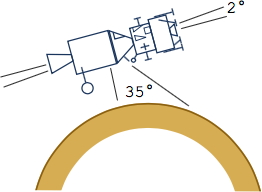
\includegraphics[width=.55\columnwidth]{images/landing4}
\end{center}


\subsection*{Heart Melt Cafe}
\begin{description}[leftmargin=6em,noitemsep,style=nextline]
	\item[Camp:] Headroom Camp
    \item[Times:] Daily, 1--3\pm, 8--11\pm
\end{description}

Share a sweet and refreshing ice cream sundae with a new person! To participate take a number and wait to be served! Feel free to join the audience and witness all of the heart melting moments! (Lactose-free vegan ice cream available upon request.)


\vbox{
\subsection*{Cheese Quesedillas}
\begin{description}[leftmargin=6em,noitemsep,style=nextline]
	\item[Camp:] Camp Polite as Fuck
  \item[Times:] Daily, 6--8\pm
\end{description}

Camp Polite as Fuck makes its glorious return To The Moon with cheese quesadillas! We will be serving daily from 6\pm--8\pm! Come by and seek refuge from the sun or in the evening if you want chill times! We love our volunteers - show us your swag!
}


%%
%%
%%
\columnbreak
\section*{Thursday, June 14, 2018}
\vbox{
\subsection*{Morning Yoga and Meditation}
\begin{description}[leftmargin=6em,noitemsep,style=nextline]
	\item[Camp:] Acrodesiac Lunartics
  \item[Times:] 9\am
\end{description}

Join us in the shade under our large AcroSpace Jam canopy for a morning yoga flow and meditation. Each day the format and style will differ as we offer various asana classes, yoga nidra, partner yoga, and more. Classes will have a different instructor each day. Meditation will be lead by Naked Stir-fry. 


\subsection*{Sensual Four-Handed Massage}
\begin{description}[leftmargin=6em,noitemsep,style=nextline]
	\item[Camp:] Herhissensua
  \item[Times:] 3--6\pm
\end{description}

Come for a relaxing massage!


\subsection*{BodyWork and Dessert}
\begin{description}[leftmargin=6em,noitemsep,style=nextline]
	\item[Camp:] Acrodesiac Lunartics
  \item[Times:] 9\pm
\end{description}

Bodywork and Dessert is a space for healing, connecting with and supporting others in our community. Yogis, massage therapists, unicorns, fairies, and those who love to give and receive are invited to share in an evening of sensual touch. Our AcroSpace Jam will be transformed into a healing space with blankets, pillows, mats, bolsters, mood lighting, and tranquil music. In the Lounge, participants informally take turns offering and receiving massage. In our lunar lounge, we will have space for conversation and desserts. So, come reset after a long day of unpacking and setting up camp! }

\begin{center}
	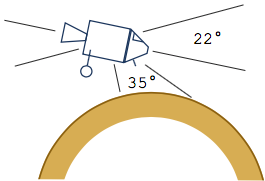
\includegraphics[width=.6\columnwidth]{images/landing3}
\end{center}

%%
%%
%%
\columnbreak
\section*{Friday, June 15, 2018}
\subsection*{Morning Yoga and Meditation}
\begin{description}[leftmargin=6em,noitemsep,style=nextline]
	\item[Camp:] Acrodesiac Lunartics
  \item[Times:] 9\am
\end{description}

Join us in the shade under our large AcroSpace Jam canopy for a morning yoga flow and meditation. Each day the format and style will differ as we offer various asana classes, yoga nidra, partner yoga, and more. Classes will have a different instructor each day. Meditation will be lead by Naked Stir-fry. 



\subsection*{Mindful Movement}
\begin{description}[leftmargin=6em,noitemsep,style=nextline]
	\item[Camp:] Neptune Ninjas
  \item[Times:] 9:30am
\end{description}

A morning mix-up of tai chi and qi gong – easy start to your day!

\subsection*{Coffee, Tea, and (G)oatmeal Social}
\begin{description}[leftmargin=6em,noitemsep,style=nextline]
	\item[Camp:] Interstellar Trill G.O.A.T.s
  \item[Times:] 10\am--12\pm
\end{description}

Interstellar Trill G.O.A.T.s, will be holding a coffee, tea, and (g)oatmeal social on Friday from 10\am--12\pm and a Moonmosa (mimosa) and Bloody Mary social on Sunday from noon-3p.

\subsection*{Sensual Four-Handed Massage}
\begin{description}[leftmargin=6em,noitemsep,style=nextline]
	\item[Camp:] Herhissensua
  \item[Times:] 10\am--4\pm
\end{description}

Come for a relaxing massage!

\subsection*{Ayurvedic Yoga Workshop}
\begin{description}[leftmargin=6em,noitemsep,style=nextline]
	\item[Camp:] The Dreamweaver Manifestation Station
    \item[Times:] 10\am--ish
\end{description}

Trying to reach balance in your life? Need to stop emotional eating, have digestive issues due to stress, monitor your health, get a fresh start?
This workshop is about using the science of Ayurvedic medicine and healing to repair digestive issues and elevate ones mood.

What you will learn:\\
What is Ayurveda\\
Understanding how Meats, sweets and wheats effect the body\\
Your personal dietary needs for your present state of health. 

This will be all levels including breath work and meditation.

Nightly before the festivities We will do a meditation as a group to set the evenings play with connection and awareness.
% \todo[inline]{google doc: Yoga workshop, based on the elemental parts of our life and our body~ fire, air, water and earth. Discussing health, lifestyle, healing both internally and physically. Included are some food tastings and some fun explorations that go perfectly with the theme of the burn.
% }

\subsection*{Tai Chi}
\begin{description}[leftmargin=6em,noitemsep,style=nextline]
	\item[Camp:] Neptune Ninjas
  \item[Times:] 10:30\am
\end{description}

Sleep in and join us for cloud hands, parting wild horses’ manes, and burning waves (our TTM invention). 

\subsection*{AcroYoga Jam}
\begin{description}[leftmargin=6em,noitemsep,style=nextline]
	\item[Camp:] Acrodesiac Lunartics
  \item[Times:] 12--6\pm
\end{description}

Join us at the AcroSpace Jam Tent at Acrodesiac Lunaratics camp for AcroYoga play. We will be offering Informal playtime all day, so don't be shy! Find any member of our camp to fly, base, and spot. Don't know what to do? We will teach you! Flow props are also  welcome and some provided.

\subsection*{Brownie Brothel}
\begin{description}[leftmargin=6em,noitemsep,style=nextline]
	\item[Camp:] Brownie Brothel
  \item[Times:] 12--6\pm
\end{description}

"Fuck your waistline," call the denizens of the Brownie Brothel, purveyors of the most titillating gourmet baked goods this side of Default Camp! Come by our boulangerie of iniquity to hang out and consume too many calories regardless of your dietary restrictions! We've got you covered. And if ya wanna, let your friendly neighborhood cookie pimps teach you a little brownie-based lesson about how sexy consent can be. Come by for dessert any time. Full-service available Friday/Saturday noon-6pm or by appointment. We'll leave the red light on for you.
(Note: Brownie Brothel is open to give away baked goods virtually any time from Thursday through Sunday, as long as someone is in camp.)

\subsection*{River Safety}
\begin{description}[leftmargin=6em,noitemsep,style=nextline]
	\item[Location:]  Riverfront below \gls{dpw}
  \item[Times:] 1:30\pm
\end{description}

\Gls{ttm} is offering a river safety class that is open to all!


\includegraphics[width=\columnwidth]{images/riversafety.png}

\subsection*{Ninja Noodle Battle}
\begin{description}[leftmargin=6em,noitemsep,style=nextline]
	\item[Camp:] Neptune Ninjas
  \item[Times:] 2:30\pm
\end{description}

For the past couple of years, water noodles and floats have battled for planetary dominance. Bring it on!

\subsection*{Tits and Tuna Party}
\begin{description}[leftmargin=6em,noitemsep,style=nextline]
	\item[Camp:] Pussy Palace
    \item[Times:] 3--6\pm
\end{description}

Feeline Frisky? Come play with all the kitties at the Pussy Palace, find your way through the Crawl Maze, and join us for the 3rd annual Tits and Tuna Party! We will be serving vegan sushi off bangin' boobies in the luxurious Velvet Pussy Dome. Fresh ahi tuna poke bowl for the carniverous cats and velvet pussy cocktails for all your feline delights!  Located at the Pussy Palace cat tower near Headroom. 

\subsection*{BLUE Party}
\begin{description}[leftmargin=6em,noitemsep,style=nextline]
	\item[Camp:] Neptune Ninjas
  \item[Times:] 5--7\pm
\end{description}

Let’s celebrate Larry’s life and his new adventure in the cosmos! Toast with Poseidon’s Punch @6.  Bring a cup and wear something blue.

\subsection*{Ministry of Silly Dance}
\begin{description}[leftmargin=6em,noitemsep,style=nextline]
	\item[Camp:] Ra!
    \item[Times:] 5--7\pm
\end{description}

It's a SILLY DANCE PARTY y'all!! Do you like shots?? Do you like Spinning wheels?? Do you like to dance as silly as possible to silly dance songs?? If you answered YES to any of these questions, then this is the game for you!! Don your extra silly gear and come bust out to your silliest dance moves with us to silly songs by artists such as Ke\$ha, James Brown, B-52's, etc!! Then take your chances and spin the Wheel of Drunk to see what shot you get as your prize!! Don't be shy! The sillier you are, the better!!  

(21+ ONLY - please have ID ready!)

\subsection*{Hearty Beef Stew}
\begin{description}[leftmargin=6em,noitemsep,style=nextline]
	\item[Camp:] Camp Homeskool
  \item[Times:] 7\pm
\end{description}

Camp Homeskool will be serving hearty beef stew Friday night around 7p.m.  Bring your own bowl and spoon like all real burners know to do.  

\subsection*{Mermaid Oasis Opening Ceremony}
\begin{description}[leftmargin=6em,noitemsep,style=nextline]
	\item[Camp:] Mermaid Oasis
  \item[Times:] 7\pm
\end{description}

Put your fins on and swim over to the Mermaid Oasis to co-create an opening ceremony to harness our magic and bless the water that we will share and drink throughout the burn. Together we will build and activate a crystal grid that we will surround with your prayer flags.  If you miss this ceremony, please stop by anytime this weekend and add your prayer flag to the mandala. All prayer flag ties will be brought to the temple burn on Sunday night

\subsection*{Karaoke and Bunless Hotdogs}
\begin{description}[leftmargin=6em,noitemsep,style=nextline]
	\item[Camp:] Camp Discordia
  \item[Times:] 8\pm
\end{description}

\subsection*{Jump in your space suit}
\begin{description}[leftmargin=6em,noitemsep,style=nextline]
	\item[Camp:] Burnning Yacht Club
  \item[Times:] 8--10\pm
\end{description}

Grab your crew get ready for blast off >>>>>TO THE MOOOOOONNN!
You and your team are venturing to the moon to collect samples and protect each other inside my blacklight moon landing photo booth!
 
Grab some of our props and samples and jump in the booth for photo shoot fuuun. Bring a phone for me to snap or take a print out of your lunar evedince. 

\vbox{
\subsection*{Special Event: Kinky Massage}
\begin{description}[leftmargin=6em,noitemsep,style=nextline]
	\item[Camp:] 
  \item[Times:] 8\pm--?
\end{description}

Ground yourself with the elements of kink through a four handed massage. Choose your yum from a menu of the senses. Try the flow of hot wax, the gust and thud of a leather flogger, the heat of fire cupping, or the restraint of hemp. We welcome all consent lovers...bring your Hell Yes!
}

\vbox{
\subsection*{Euphoria \Gls{temple} Burn}
\begin{description}[leftmargin=6em,noitemsep,style=nextline]
	\item[Location:] Burn site
  \item[Times:] O'Dark Thirty
\end{description}

This is a special temple burn for this year's \gls{ttm}.  The Euphoria burn has kindly donated their \gls{temple} that was to be burned at their abruptly canceled event to \gls{ttm} to be burned on Friday night at \gls{ttm}.

The Euphoria \Gls{temple} was built by Patrick Murphy and Katie Herman.
}

\vbox{
\subsection*{Hippie Cooker}
\begin{description}[leftmargin=6em,noitemsep,style=nextline]
	\item[Camp:] Camp Homeskool
  \item[Times:] late night
\end{description}

Once again we will have our Hippie Cooker (propane-fired sauna) up and running late Friday and Saturday nights and  Saturday morning to sweat out your toxins. Come join us.
}

\begin{center}
	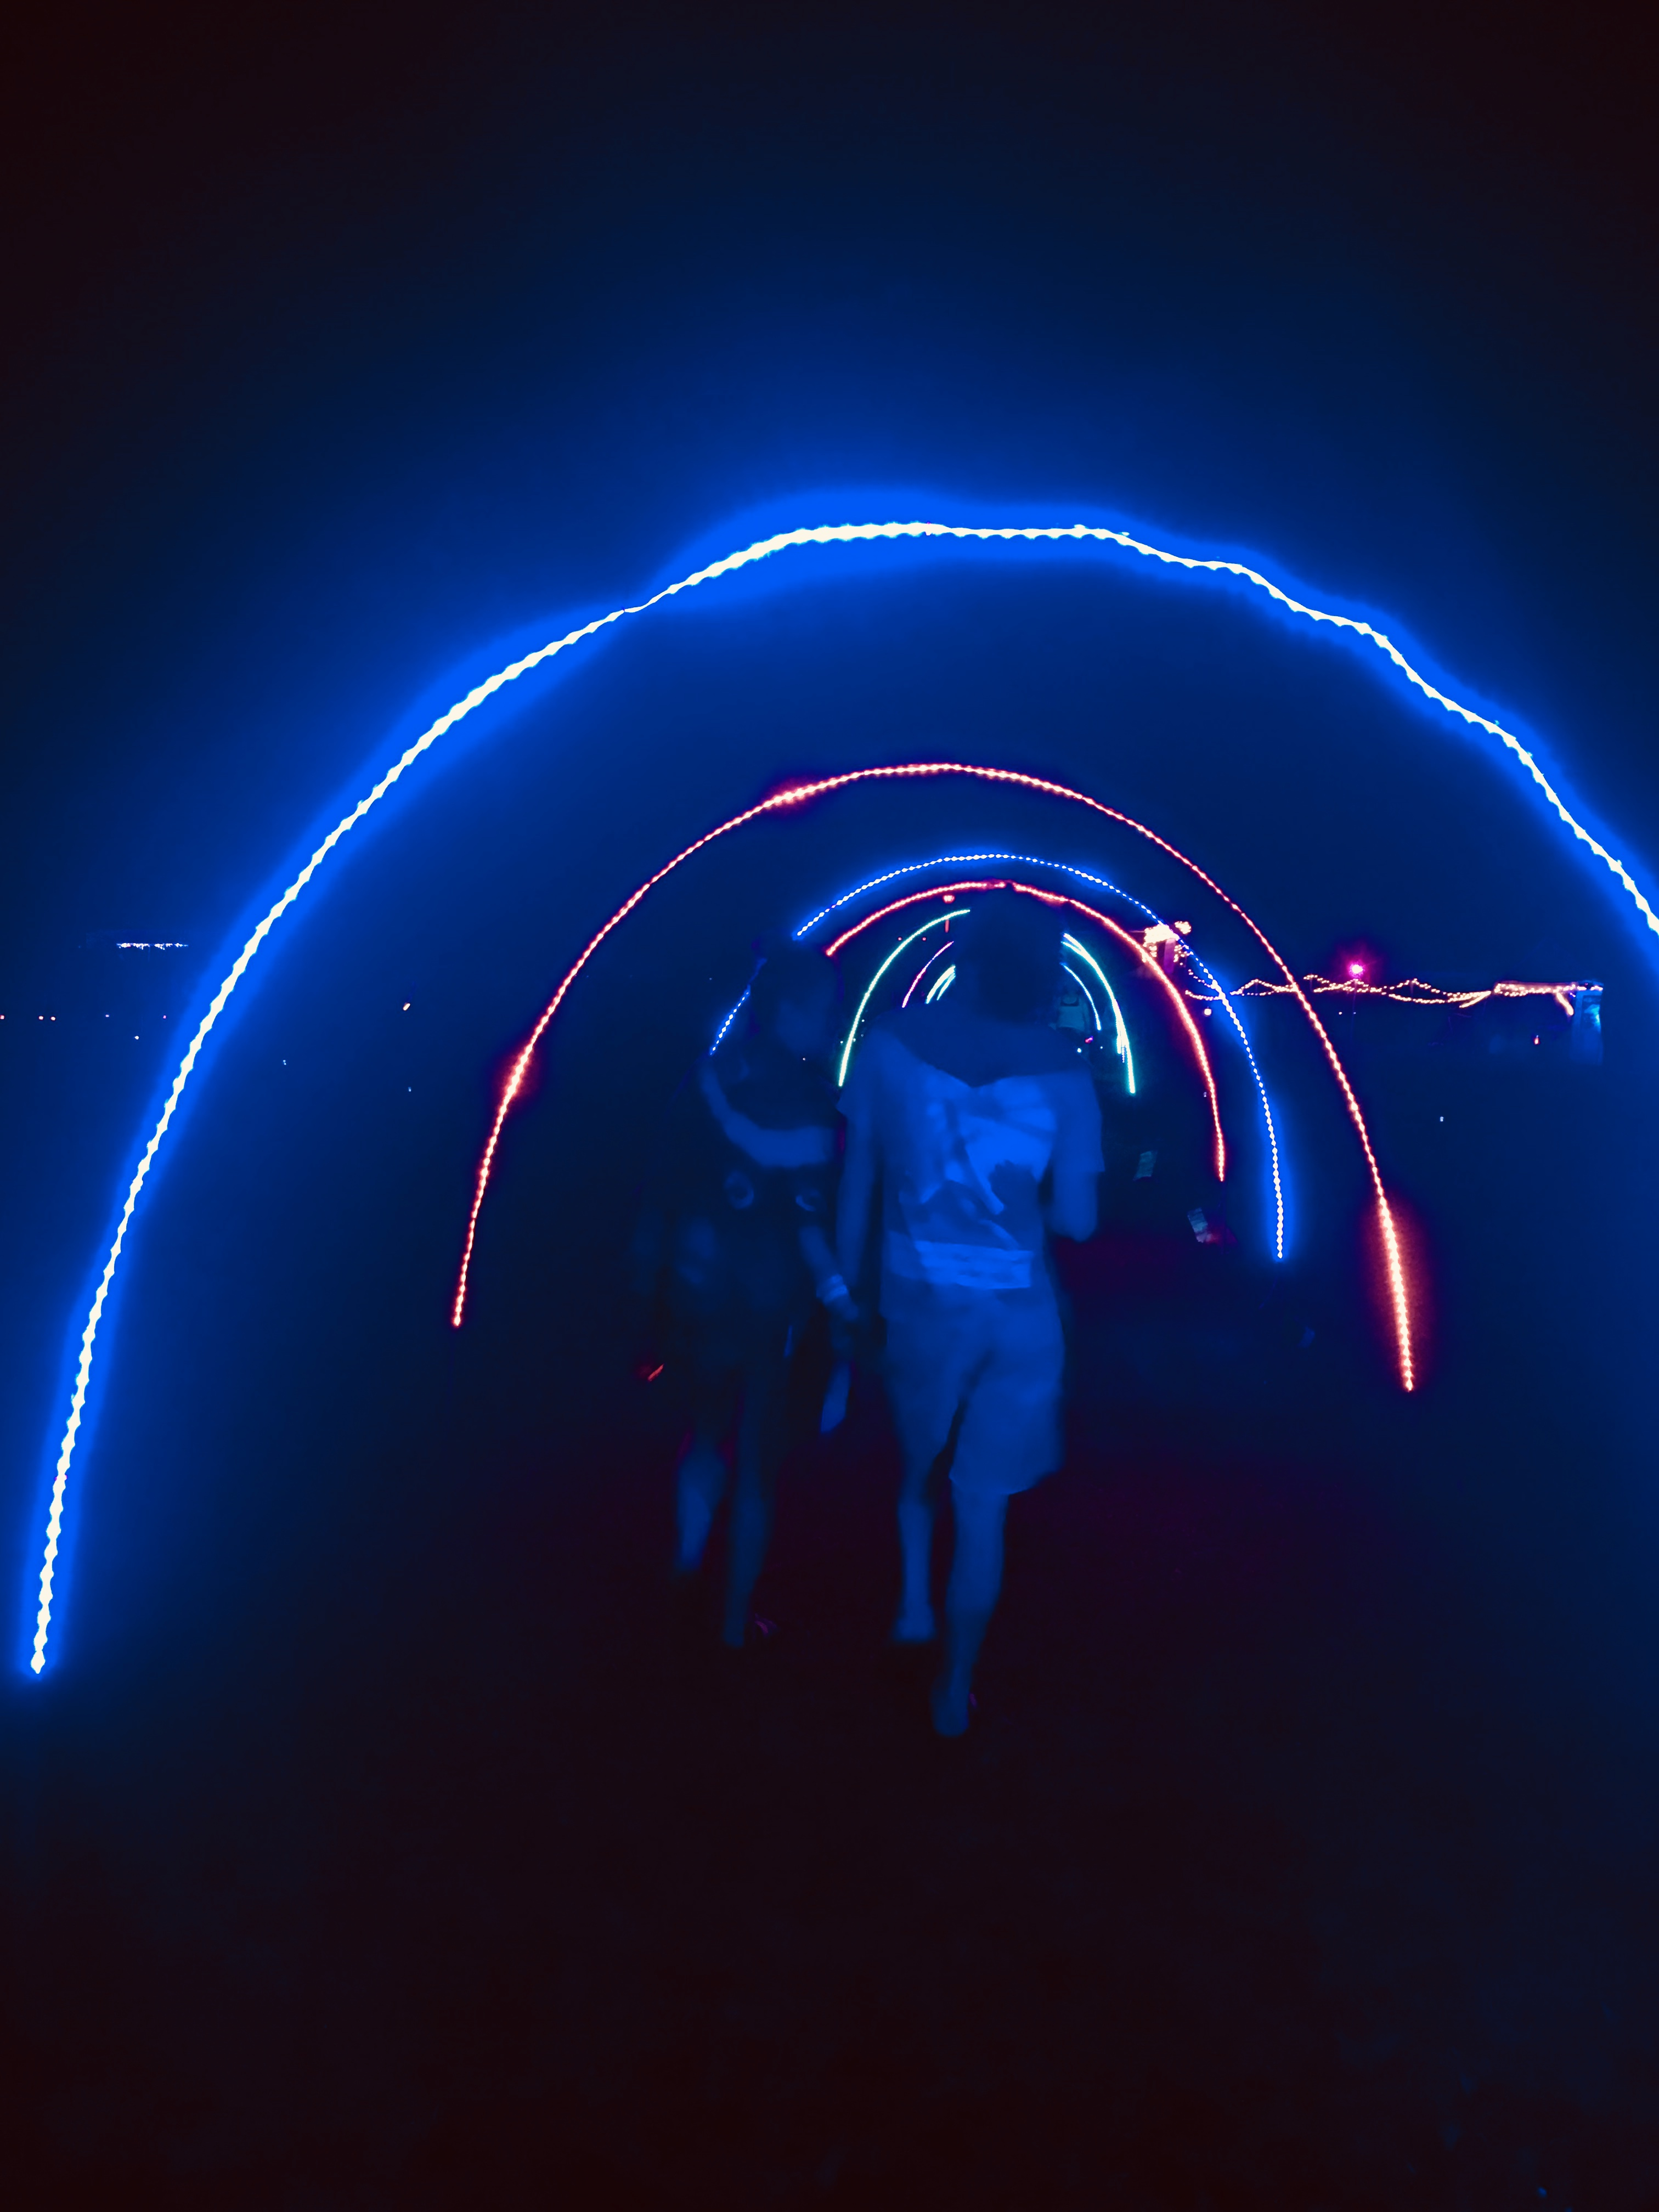
\includegraphics[width=\columnwidth]{images/TTM2017tunnel}
    \label{image:tunnel}
\end{center}

%%
%%
%%
\columnbreak
\section*{Saturday, June 16, 2018}
\subsection*{Hippie Cooker}
\begin{description}[leftmargin=6em,noitemsep,style=nextline]
	\item[Camp:] Camp Homeskool
  \item[Times:] morning
\end{description}

Once again we will have our Hippie Cooker (propane-fired sauna) up and running late Friday and Saturday nights and  Saturday morning to sweat out your toxins. Come join us.

\subsection*{Breakfast Burritos}
\begin{description}[leftmargin=6em,noitemsep,style=nextline]
	\item[Camp:] Camp Homeskool
  \item[Times:] 7\pm
\end{description}

Camp Homeskool will be serving up breakfast burritos around 9a.m.

\subsection*{Morning Yoga and Meditation}
\begin{description}[leftmargin=6em,noitemsep,style=nextline]
	\item[Camp:] Acrodesiac Lunartics
  \item[Times:] 9\am
\end{description}

Join us in the shade under our large AcroSpace Jam canopy for a morning yoga flow and meditation. Each day the format and style will differ as we offer various asana classes, yoga nidra, partner yoga, and more. Classes will have a different instructor each day. Meditation will be lead by Naked Stir-fry. 


\subsection*{Mindful Movement}
\begin{description}[leftmargin=6em,noitemsep,style=nextline]
	\item[Camp:] Neptune Ninjas
  \item[Times:] 9:30\am
\end{description}

A morning mix-up of tai chi and qi gong – easy start to your day!

\subsection*{Ayurvedic yoga workshop}
\begin{description}[leftmargin=6em,noitemsep,style=nextline]
	\item[Camp:] The Dreamweaver Manifestation Station
    \item[Times:] 10\am--ish
\end{description}

Trying to reach balance in your life? Need to stop emotional eating, have digestive issues due to stress, monitor your health, get a fresh start?
This workshop is about using the science of Ayurvedic medicine and healing to repair digestive issues and elevate ones mood.

What you will learn:
What is Ayurveda
Understanding how Meats, sweets and wheats effect the body
Your personal dietary needs for your present state of health. 

This will be all levels including breath work and meditation.

Nightly before the festivities We will do a meditation as a group to set the evenings play with connection and awareness.

\subsection*{Sensual Four-Handed Massage}
\begin{description}[leftmargin=6em,noitemsep,style=nextline]
	\item[Camp:] Herhissensua
  \item[Times:] 10\am--4\pm
\end{description}

Come for a relaxing massage!

\subsection*{Tai Chi}
\begin{description}[leftmargin=6em,noitemsep,style=nextline]
	\item[Camp:] Neptune Ninjas
  \item[Times:] 10:30\am
\end{description}

Sleep in and join us for cloud hands, parting wild horses’ manes, and burning waves (our TTM invention). 

\subsection*{Yin Yoga Flow with Meryl }
\begin{description}[leftmargin=6em,noitemsep,style=nextline]
	\item[Location:] Near the \gls{temple}
  \item[Times:] 11\am
\end{description}

Let's greet the day with Slow Flow Yin Yoga in the mist. Bring a blanket, mat or towel, and move with us for a perfect way to start Burn Day! 
Find our circle near temple! 

\subsection*{Disco Brunch}
\begin{description}[leftmargin=6em,noitemsep,style=nextline]
	\item[Camp:] Headroom
    \item[Times:] 12--2\pm
\end{description}

Disco and Mimosas served aboard the Struggle Bus. The Disco Brunch has been held annually since Alchemy 2012 and is always guaranteed to be a good day party with appropriate music and of course.... champagne!!!

\subsection*{Brownie Brothel}
\begin{description}[leftmargin=6em,noitemsep,style=nextline]
	\item[Camp:] Brownie Brothel
  \item[Times:] 12--6\pm
\end{description}

"Fuck your waistline," call the denizens of the Brownie Brothel, purveyors of the most titillating gourmet baked goods this side of Default Camp! Come by our boulangerie of iniquity to hang out and consume too many calories regardless of your dietary restrictions! We've got you covered. And if ya wanna, let your friendly neighborhood cookie pimps teach you a little brownie-based lesson about how sexy consent can be. Come by for dessert any time. Full-service available Friday/Saturday noon-6pm or by appointment. We'll leave the red light on for you.
(Note: Brownie Brothel is open to give away baked goods virtually any time from Thursday through Sunday, as long as someone is in camp.)

\subsection*{Story Telling and Singing}
\begin{description}[leftmargin=6em,noitemsep,style=nextline]
	\item[Camp:] Camp Homeskool
  \item[Times:] 7\pm
\end{description}

Camp Homeskool will have story telling and singing with Uncle Mike. (Yes this really is a kid friendly event for our junior burners.)   

\subsection*{Ninja Noodle Battle}
\begin{description}[leftmargin=6em,noitemsep,style=nextline]
	\item[Camp:] Neptune Ninjas
  \item[Times:] 2:30\pm
\end{description}

For the past couple of years, water noodles and floats have battled for planetary dominance. Bring it on!

\columnbreak
\subsection*{AcroYoga Jam}
\begin{description}[leftmargin=6em,noitemsep,style=nextline]
	\item[Camp:] Acrodesiac Lunartics
  \item[Times:] 3--6\pm
\end{description}

Join us at the AcroSpace Jam Tent at Acrodesiac Lunaratics camp for AcroYoga play. We will be offering Informal playtime all day, so don't be shy! Find any member of our camp to fly, base, and spot. Don't know what to do? We will teach you! Flow props are also  welcome and some provided.

\subsection*{Ministry of Silly Dance}
\begin{description}[leftmargin=6em,noitemsep,style=nextline]
	\item[Camp:] Ra!
    \item[Times:] 3--5\pm
\end{description}

It's a SILLY DANCE PARTY y'all!! Do you like shots?? Do you like Spinning wheels?? Do you like to dance as silly as possible to silly dance songs?? If you answered YES to any of these questions, then this is the game for you!! Don your extra silly gear and come bust out to your silliest dance moves with us to silly songs by artists such as Ke\$ha, James Brown, B-52's, etc!! Then take your chances and spin the Wheel of Drunk to see what shot you get as your prize!! Don't be shy! The sillier you are, the better!!  

(21+ ONLY - please have ID ready!)

\subsection*{Mehndi Art}
\begin{description}[leftmargin=6em,noitemsep,style=nextline]
	\item[Camp:] Neptune Ninjas
  \item[Times:] 3:30\pm
\end{description}

Let’s play with henna and decorate ourselves!

\subsection*{Animal Totem Readings}
\begin{description}[leftmargin=6em,noitemsep,style=nextline]
	\item[Camp:] Neptune Ninjas
  \item[Times:] 4:15\pm
\end{description}

Discover your TTM Spirit animal. Let them guide you on your celestial TTM journey!

\columnbreak
\subsection*{Labyrinth Walk}
\begin{description}[leftmargin=6em,noitemsep,style=nextline]
	\item[Camp:] Neptune Ninjas
  \item[Times:] 5\pm
\end{description}

Take your shoes off and free your spirit with a walk about a labyrinth!


\subsection*{Planetary Bead Charms}
\begin{description}[leftmargin=6em,noitemsep,style=nextline]
	\item[Camp:] Neptune Ninjas
  \item[Times:] 6\pm
\end{description}

Feel like making a bracelet to honor your favorite planet or all of them – join us for some beading.

\subsection*{Jump in your space suit}
\begin{description}[leftmargin=6em,noitemsep,style=nextline]
	\item[Camp:] Burnning Yacht Club
  \item[Times:] 8--10\pm
\end{description}

Grab your crew get ready for blast off >>>>>TO THE MOOOOOONNN!
You and your team are venturing to the moon to collect samples and protect each other inside my blacklight moon landing photo booth!
 
Grab some of our props and samples and jump in the booth for photo shoot fuuun. Bring a phone for me to snap or take a print out of your lunar evedince. 

\subsection*{Effigy Burn}
\begin{description}[leftmargin=6em,noitemsep,style=nextline]
	\item[Location:] Burn site
    \item[Times:] O'Dark Thirty
\end{description}

\begin{center}
	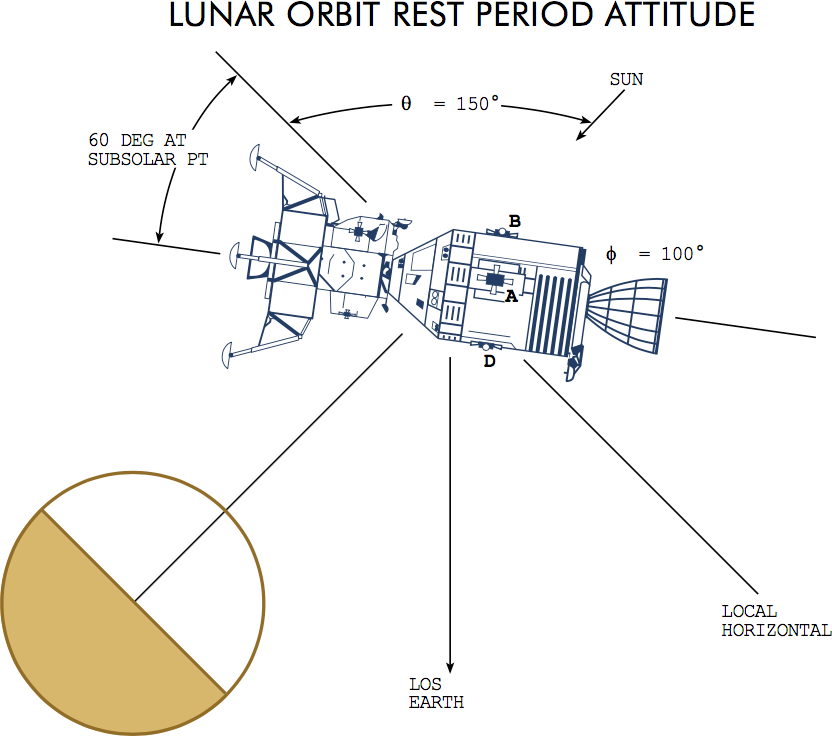
\includegraphics[width=.8\columnwidth]{images/lunarorbitrestperiod}
\end{center}

\vbox{
\subsection*{Hippie Cooker}
\begin{description}[leftmargin=6em,noitemsep,style=nextline]
	\item[Camp:] Camp Homeskool
  \item[Times:] late night
\end{description}

Once again we will have our Hippie Cooker (propane-fired sauna) up and running late Friday and Saturday nights and  Saturday morning to sweat out your toxins. Come join us.
}


\vspace*{\fill}

% multicols NO LIKEE FLOATS  :-(
% \begin{figure}[h!]
% \centering
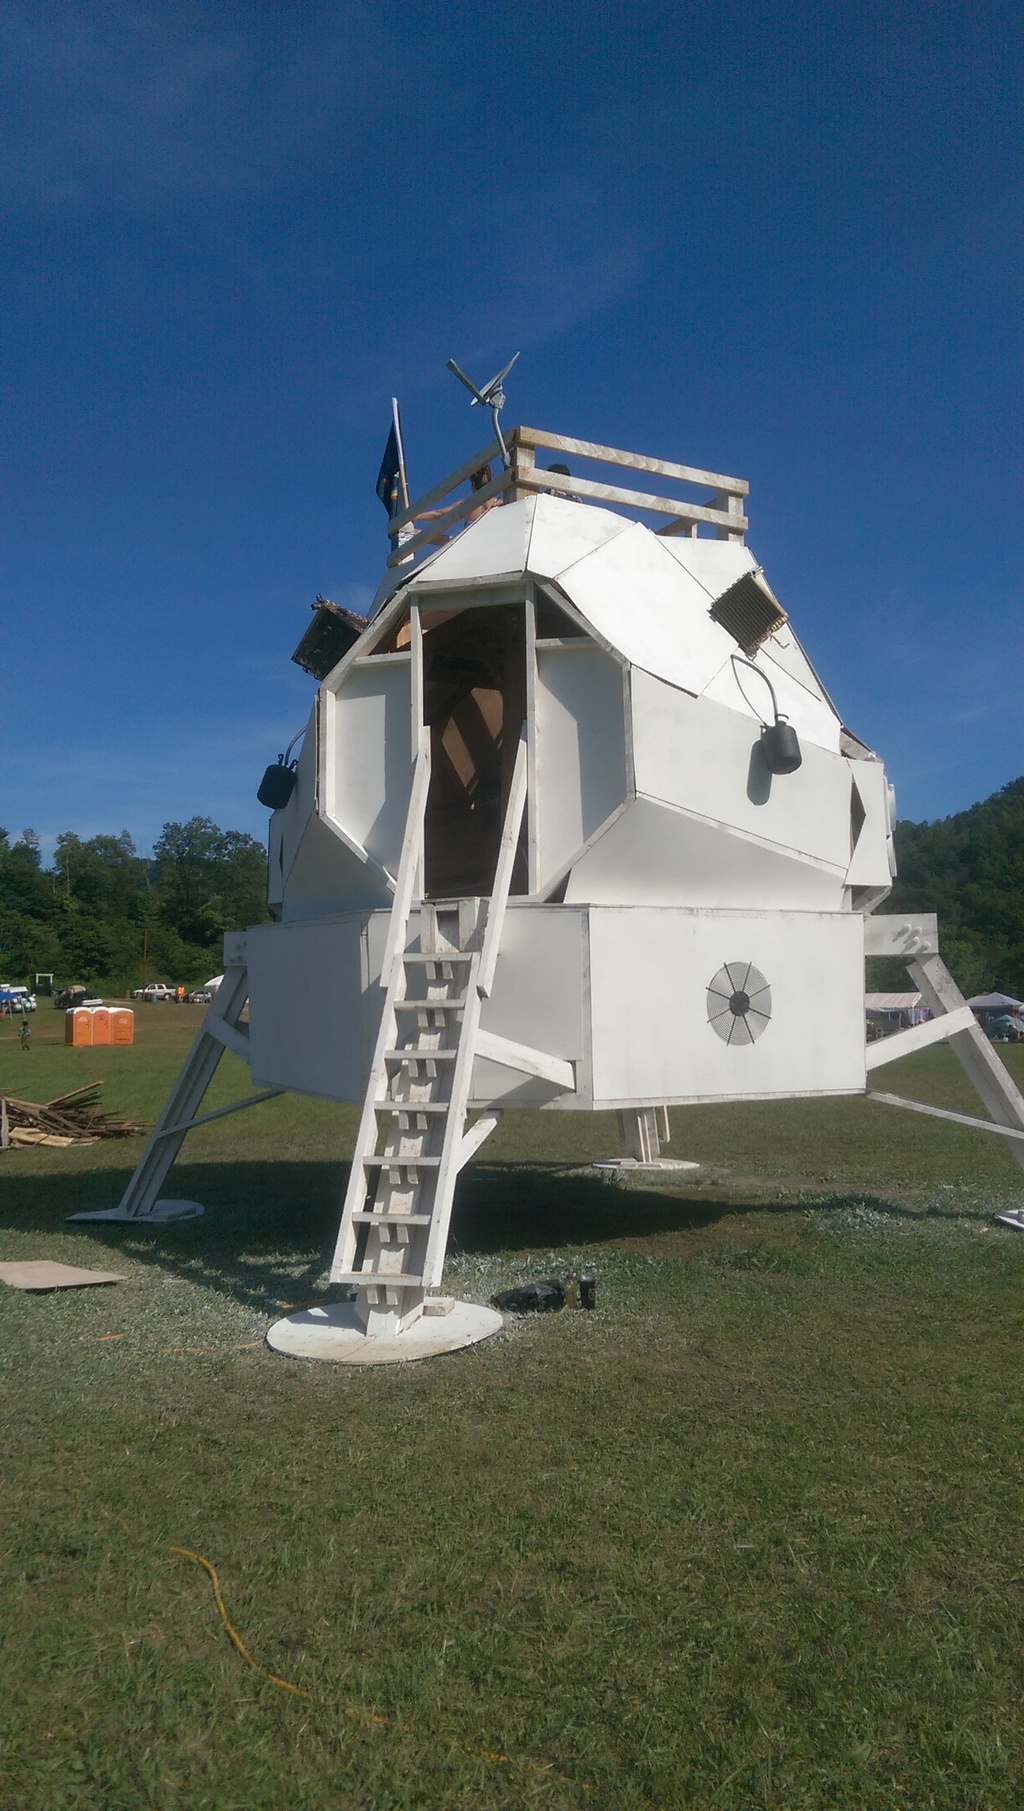
\includegraphics[width=\columnwidth]{images/2017Effigy_small}
% \caption{\label{fig:2017effigy} Crew inspecting the 2017 effigy before its final launch.}
% \end{figure}
\vspace*{\fill}

%%
%%
%%
\columnbreak
\section*{Sunday, June 17, 2018}
\subsection*{Morning Yoga and Meditation}
\begin{description}[leftmargin=6em,noitemsep,style=nextline]
	\item[Camp:] Acrodesiac Lunartics
  \item[Times:] 9\am
\end{description}

Join us in the shade under our large AcroSpace Jam canopy for a morning yoga flow and meditation. Each day the format and style will differ as we offer various asana classes, yoga nidra, partner yoga, and more. Classes will have a different instructor each day. Meditation will be lead by Naked Stir-fry. 

\subsection*{Mindful Movement}
\begin{description}[leftmargin=6em,noitemsep,style=nextline]
	\item[Camp:] Neptune Ninjas
  \item[Times:] 9:30\am
\end{description}

A morning mix-up of tai chi and qi gong – easy start to your day!

\subsection*{Tai Chi}
\begin{description}[leftmargin=6em,noitemsep,style=nextline]
	\item[Camp:] Neptune Ninjas
  \item[Times:] Friday--Sunday 10:30\am
\end{description}

Sleep in and join us for cloud hands, parting wild horses’ manes, and burning waves (our TTM invention). 

\subsection*{Tye Dye Party}
\begin{description}[leftmargin=6em,noitemsep,style=nextline]
	\item[Camp:] Camp Homeskool
  \item[Times:] noon-ish
\end{description}

Sunday around noon we will be hosting a tye dye party for kids of all ages.

\vbox{ 
\subsection*{Open Stage}
\begin{description}[leftmargin=6em,noitemsep,style=nextline]
	\item[Camp:] Neptune Ninjas
  \item[Times:] after noon
\end{description}

After noon our camp will host your TTM talk, demo or art session. Please see Freedom to get on the schedule! We will post your topic on our board at the front of the stage as soon as you let us know what knowledge you would like to “gift” our community.
}


\subsection*{Moonmosa (mimosa) and Bloody Mary Social}
\begin{description}[leftmargin=6em,noitemsep,style=nextline]
	\item[Camp:] Interstellar Trill G.O.A.T.s
  \item[Times:] 12-3\pm
\end{description} 

\subsection*{\Gls{temple} Burn}
\vbox{
\begin{description}[leftmargin=6em,noitemsep,style=nextline]
	\item[Location:] Burn site
    \item[Times:] O'Dark Thirty
\end{description}

We would like to introduce the ElemenTemple! This is where Fire, Water, Earth and Air, join with the Spirit, brought together through an eclectic collaboration of art! This will be in the lower level. 
From the ground to the sky will be the connection of the creation, the universe and all, sending a beacon of light into the sky.
The ElemenTemple burn will be at dusk/dark:30 Sunday evening, so please plan on hanging out to send her to the skies and back.

Please feel free as always to write your dreams and wishes, anything you want to take in or let go of, and if you would like to keep them private, there will be paper to write on that will remain confidential, that I will hang in the temple before we send it up.
See ya'll on the MOOOOON!!!!

ElmenenTemple designed and built by Michael "Lunar" Luber and Matthew Horner.
}

\end{multicols}

\vspace*{\fill}
\begin{center}
	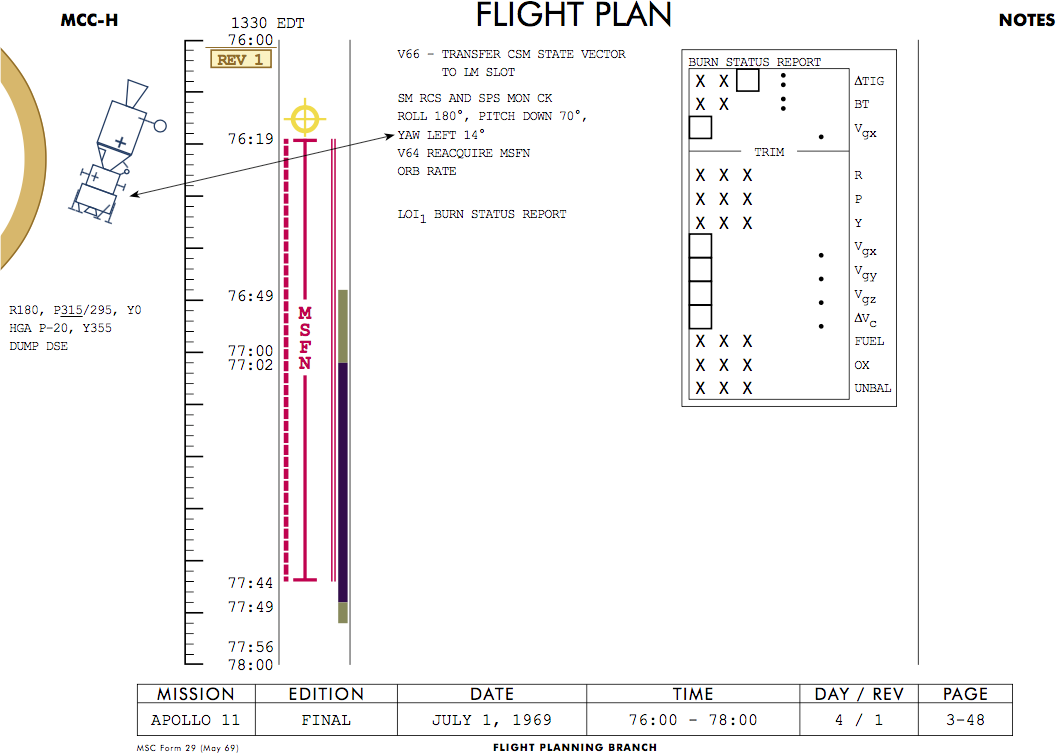
\includegraphics[width=.8\textwidth]{images/flightplan2}
\end{center}
\vspace*{\fill}

\newpage
\pagestyle{empty}
\vspace*{\fill}
\begin{center}
\texttt{THIS PAGE INTENTONALLY LEFT BLANK.}
\end{center}
\vspace*{\fill}


